%!TEX root = ../../../main.tex


\section[Antennas]{Coupling \Nds to Double Bowtie Antenna Structures} \label{sec::coupling_antennas}

	In this chapter, the integration of \sivs in nanodiamonds with double bowtie nanoantenna structures is presented.
	The emission from the coupled system has two advantages:
	\begin{itemize}
		\item The antenna causes an enhancement in the \siv{}'s \pl emission intensity.
		\item The \pl spectrum of the nanodiamond is modified depending on the geometry of the nanoantenna as well as the position of the emitter in the gap. This provides the flexibility of designing the nanoantennas to accurately predict and tune the emitters' PL spectrum as desired.
	\end{itemize}
	
	

	\begin{figure}[tp]
		\begin{subfigure}[t]{ 0.49\linewidth}
			\centering
			\testbox{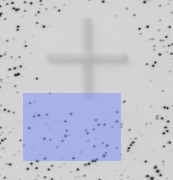
\includegraphics[trim = 0 0 0 0,  clip= true, width = \textwidth]{./pics/M05-13_structure3_stitch_crop_area.jpg}}
			\caption{}
			\label{subfig::cross_laser_scan}
		\end{subfigure}
		\hfill
		\begin{subfigure}[t]{ 0.49\linewidth}
			\centering
			\testbox{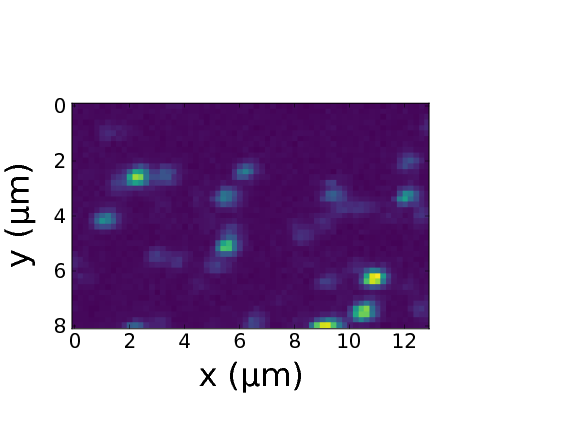
\includegraphics[trim = 0 20 70 50,  clip= true, width = \textwidth]{./pics/scan_xy-32_2APD_mum_noscale.png}}
			\caption{}
			\label{subfig::pp_pl_scan}
		\end{subfigure}
		\caption{ (a) Picture recorded with a commercial high resolution laser scanning microscope. The area shaded in blue represents the \pl scan in image (b). (b) \Pl scan of a \SI{8}{\micro\metre}x\SI{13}{\micro\metre}}
	\end{figure}


	\begin{figure}[tp]
		\begin{subfigure}[t]{ 0.49\linewidth}
			\centering
			\testbox{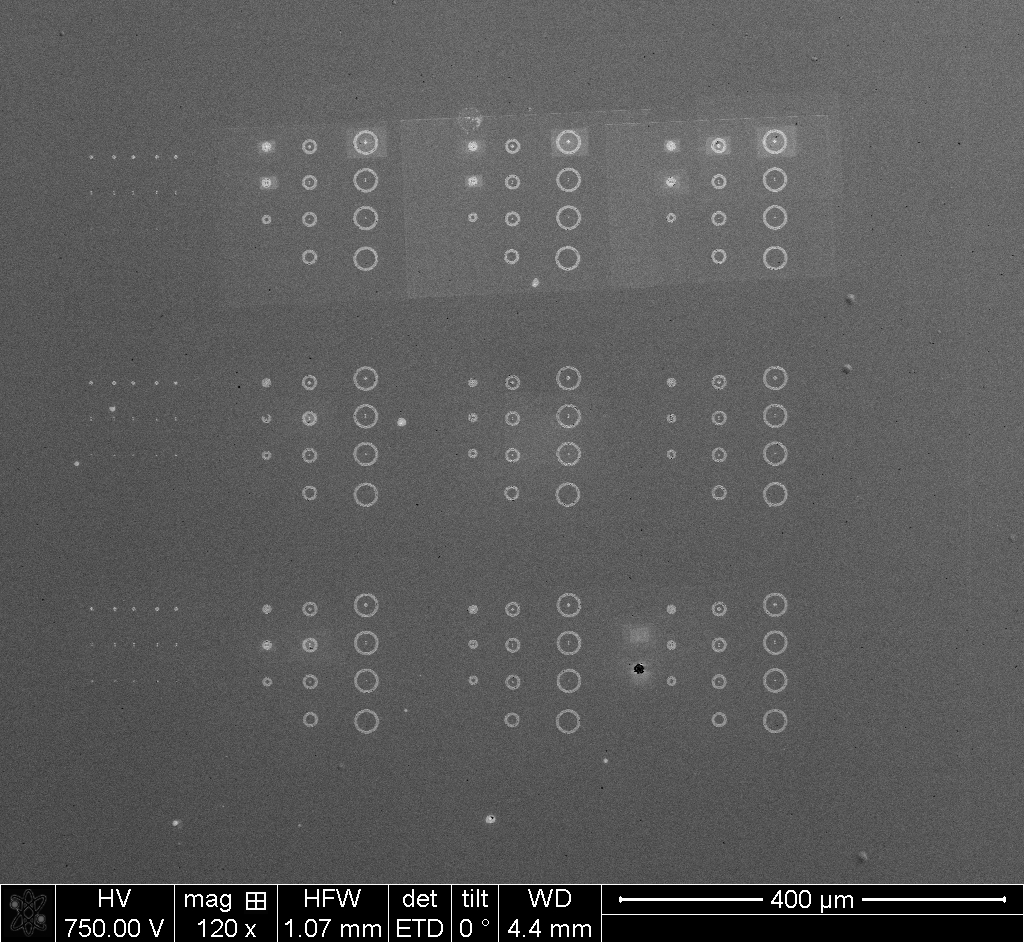
\includegraphics[trim = 0 0 0 0,  clip= true, width = \textwidth]{./pics/Antenna2_upper_right_150923_01.png}}
			\caption{<caption>}
			\label{subfig::antenna_structures_sem}
		\end{subfigure}
		\hfill
		\begin{subfigure}[t]{ 0.49\linewidth}
			\centering
			\testbox{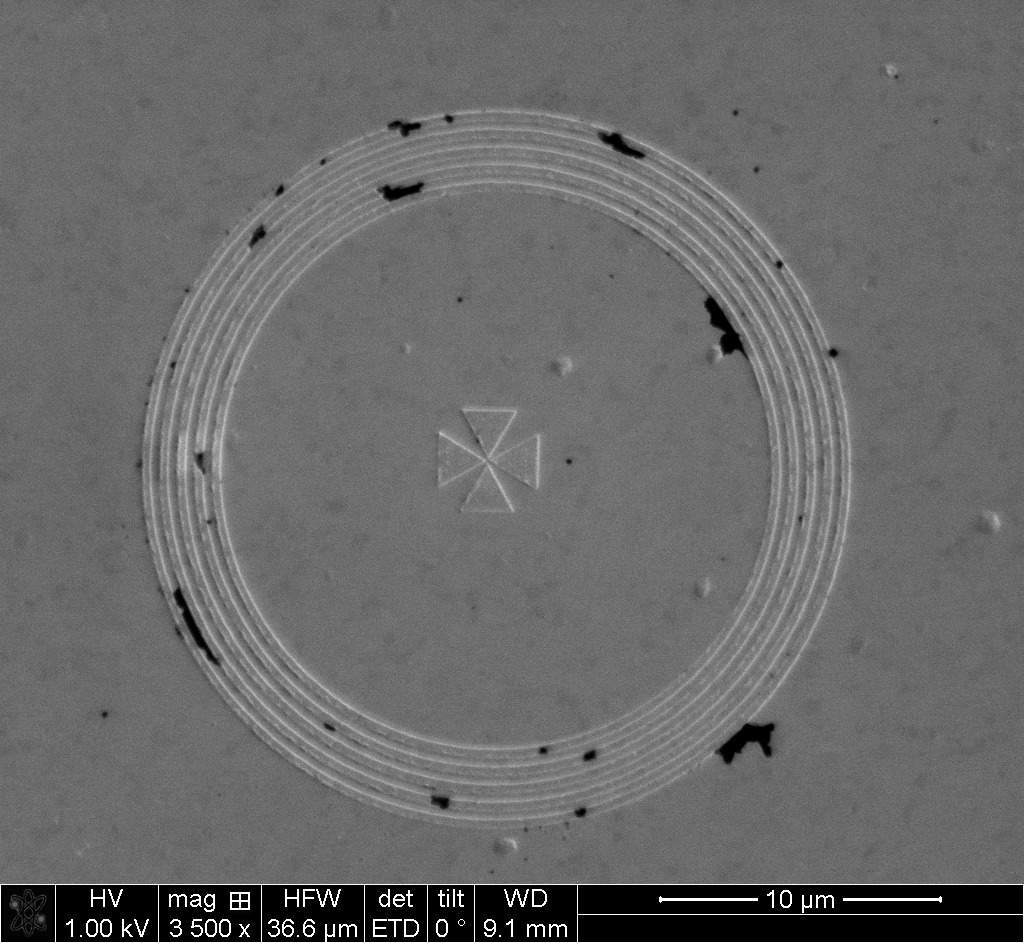
\includegraphics[trim = 0 0 0 0,  clip= true, width = \textwidth]{./pics/Ir27M_mitte_213_151111_13.jpg}}
			\caption{<caption>}
			\label{subfig::antenna_one_structure_sem}
		\end{subfigure}
		\caption{<caption>}
		\label{fig::<fig>}
	\end{figure}

	\begin{figure}[tp]
		\centering
		\testbox{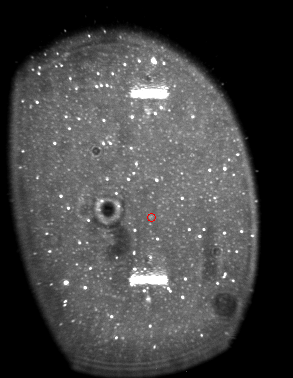
\includegraphics[trim = 0 0 0 0,  clip= true, width = 0.3\textwidth]{./pics/ccd_f301_emitter7.png}}
		\caption{Image of the sample surface of \SI{100}{nm} wet-milled nanodiamonds spin-coated on an \ir substrate illuminated with diffuse white light. The white bars are the horizontal bars of the cross markers which serve as a coarse orientation on the sample surface, the white dots are nanodiamonds, the big black spot is an artifact.}
		\label{fig::ccd_cross_marker}
	\end{figure}

	% \begin{figure}[tp]
	% 	\begin{subfigure}[t]{ 0.49\linewidth}
	% 		\centering
	% 		\testbox{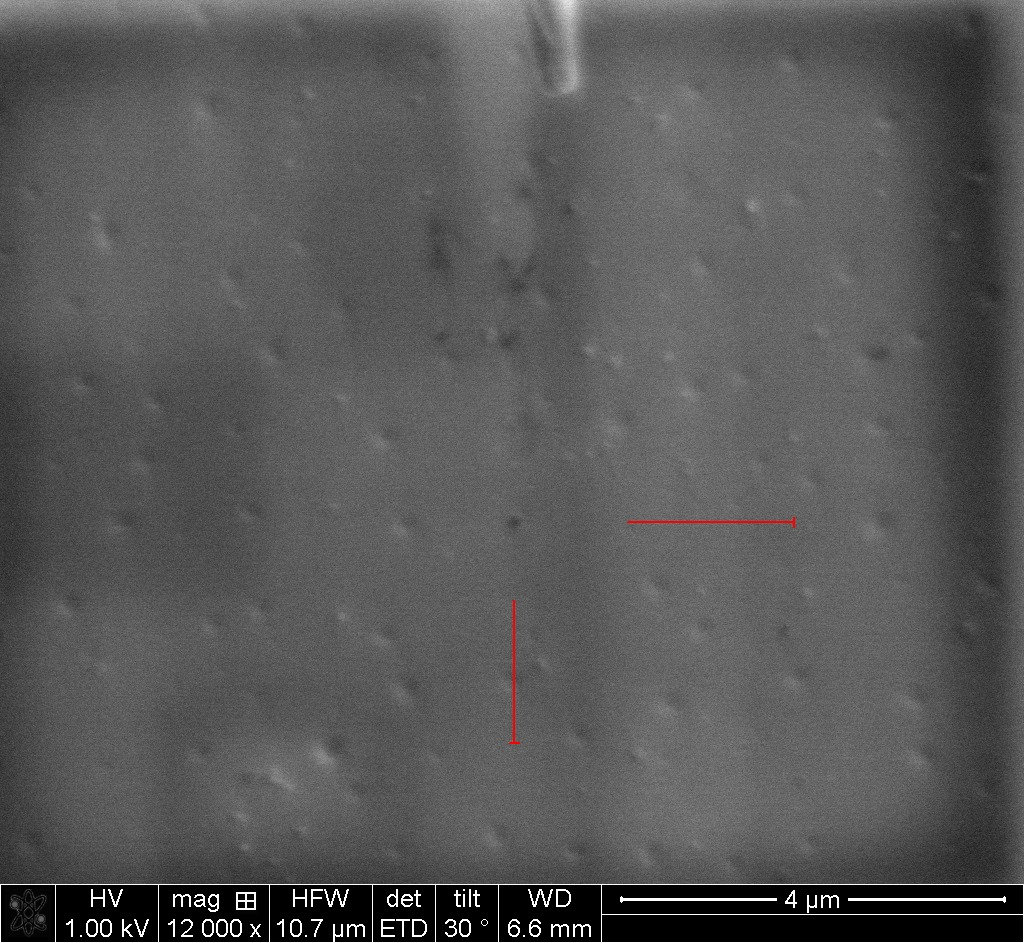
\includegraphics[trim = 0 0 0 0,  clip= true, width = \textwidth]{./pics/Ir27M_mitte_213_151111_18.jpg}}
	% 		\caption{}
	% 		\label{subfig::nd_before_pick_hr}
	% 	\end{subfigure}
	% 	\hfill
	% 	\begin{subfigure}[t]{ 0.49\linewidth}
	% 		\centering
	% 		\testbox{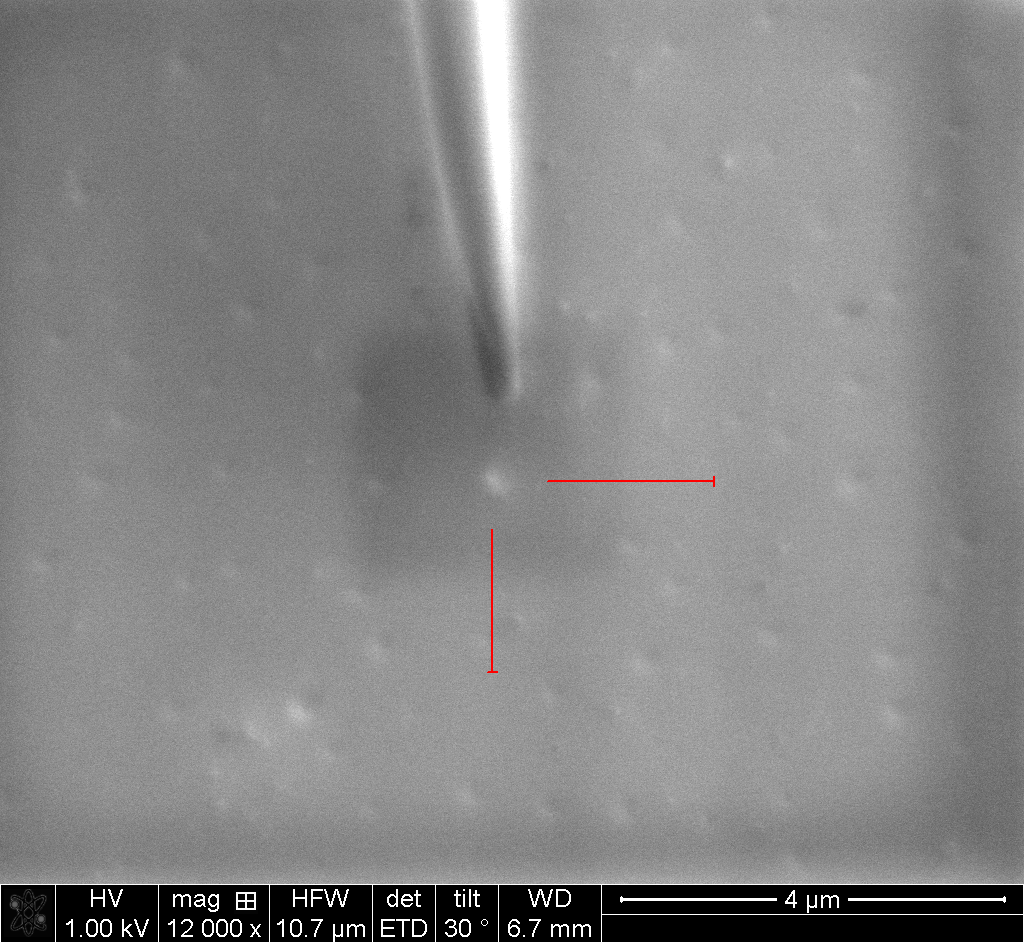
\includegraphics[trim = 0 0 0 0,  clip= true, width = \textwidth]{./pics/Ir27M_mitte_213_151111_21.png}}
	% 		\caption{}
	% 		\label{subfig::nd_before_pick_no_hr}
	% 	\end{subfigure}
	% 	\caption{caption}
	% \end{figure}

	\begin{figure}[tp]
		\begin{subfigure}[t]{ 0.49\linewidth}
			\centering
			\testbox{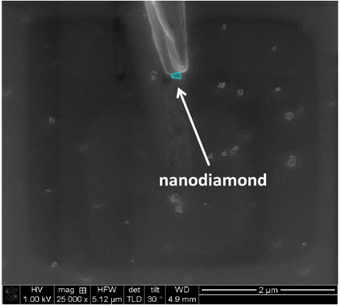
\includegraphics[trim = 0 0 0 0,  clip= true, width = \textwidth]{./pics/pick_colored.png}}
			\caption{}
			\label{subfig::pick_antenna_sem}
		\end{subfigure}
		\hfill
		\begin{subfigure}[t]{ 0.49\linewidth}
			\centering
			\testbox{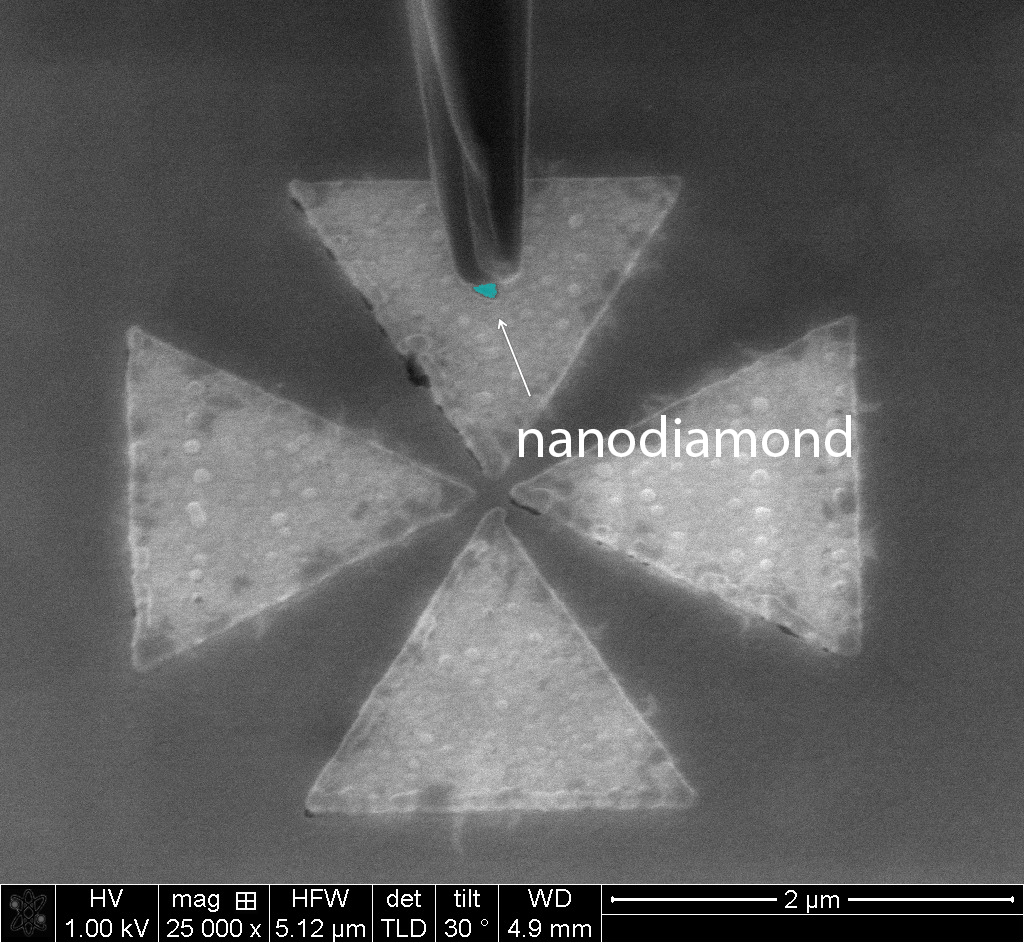
\includegraphics[trim = 0 0 0 0,  clip= true, width = \textwidth]{./pics/Ir27M_mitte_213_151111_26_colored.png}}
			\caption{}
			\label{subfig::transfer_antenna_sem}
		\end{subfigure}
		\caption{}
	\end{figure}

	\subsection{Structure of the Plasmonic Antennas} \label{sec::structure_antenna}

	\begin{figure}[tp]
		\centering
		\testbox{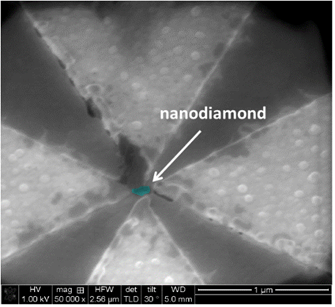
\includegraphics[trim = 0 0 0 0,  clip= true, width = 0.3\textwidth]{./pics/place_colored.png}}
		\caption{<caption>}
		\label{fig::place_antenna_sem}
	\end{figure}

	\begin{figure}[tp]
		\centering
		\testbox{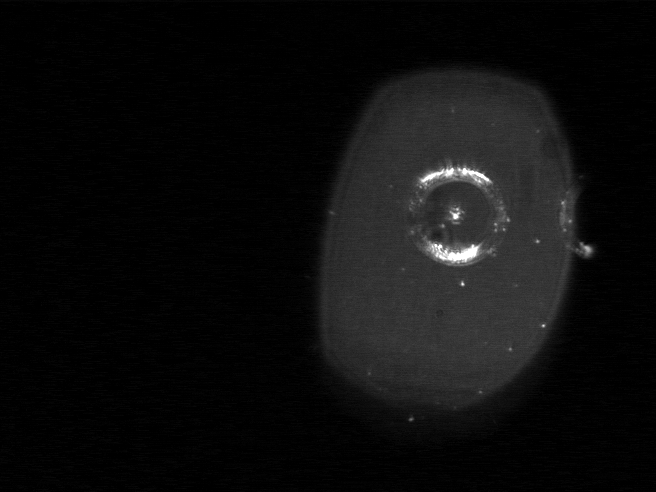
\includegraphics[trim = 120 0 0 0,  clip= true, width = 0.3\textwidth]{./pics/ccd_s1_g3_db_g150_d20_rightone.png}}
		\caption{}
		\label{fig::place_ccd}
	\end{figure}

	\begin{figure}[tp]
		\centering
		\testbox{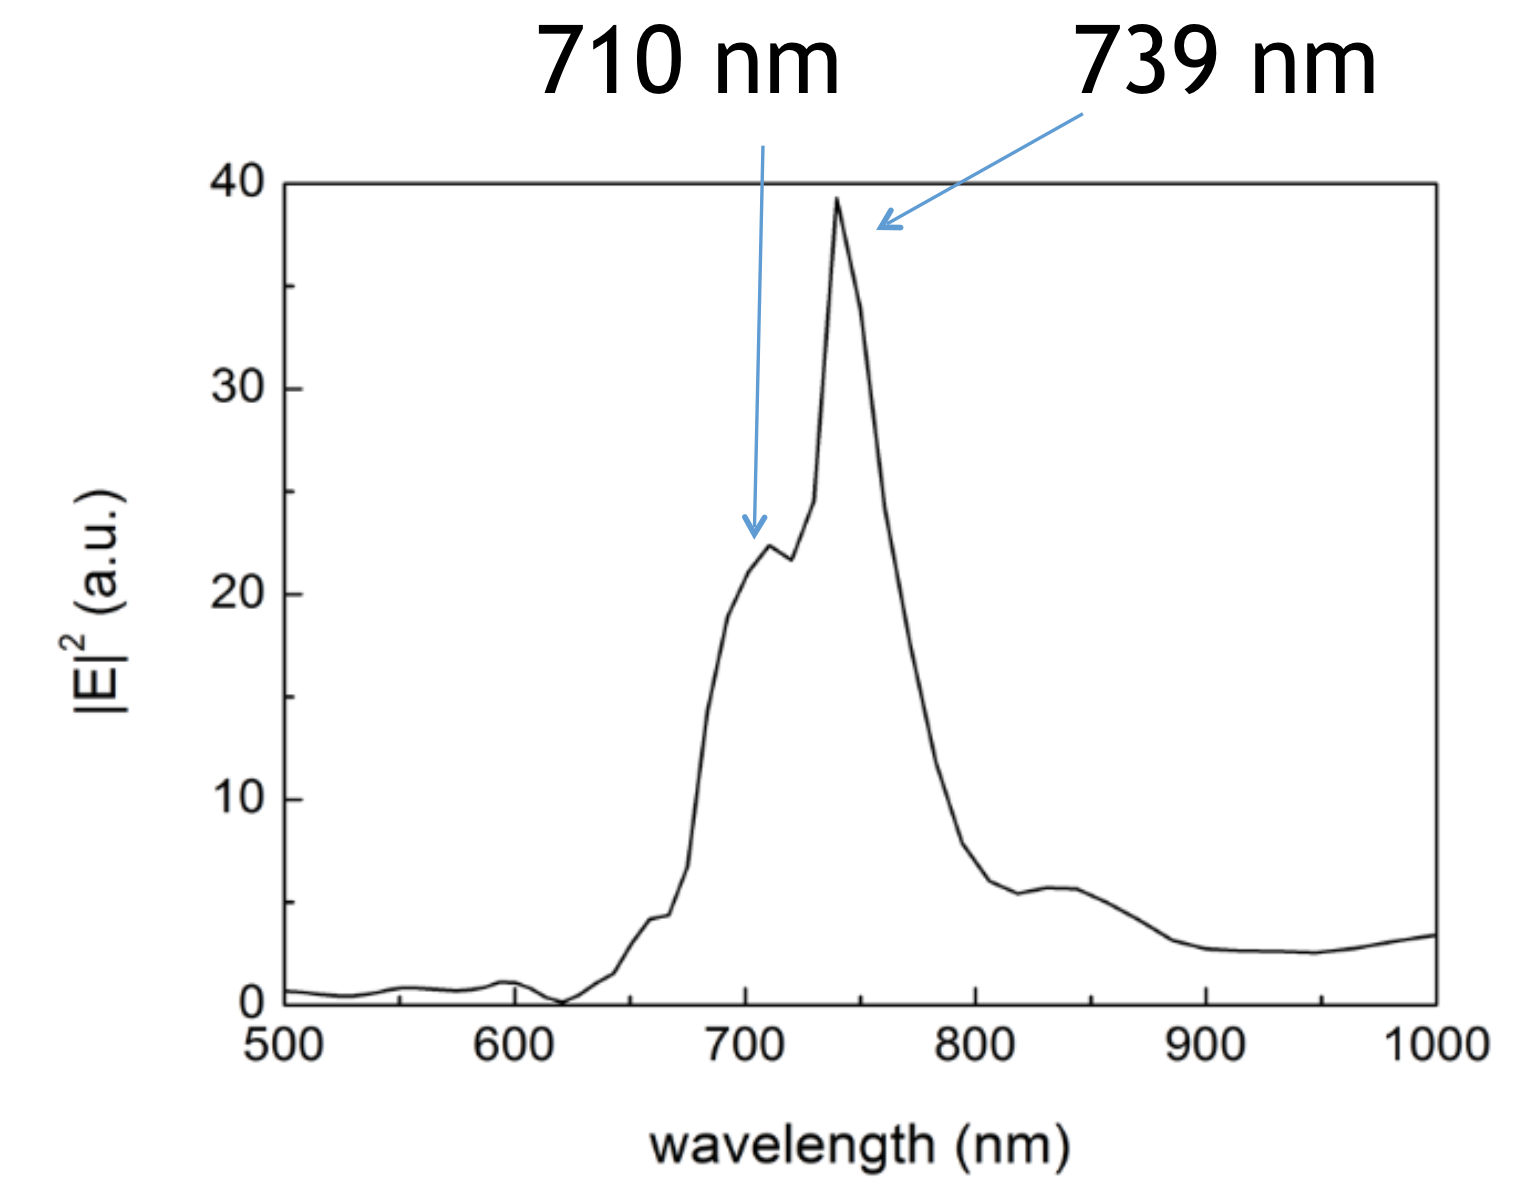
\includegraphics[trim = 0 0 0 0,  clip= true, width = 0.5\textwidth]{./pics/antenna_fdtd_calculation.png}}
		\caption{<caption>}
		\label{fig::antenna_fdtd_calculation}
	\end{figure}

	FDTD numerical simulations were performed using Lumerical software to characterize gold double bowtie nanoantennas on a gold substrate. The nanoantennas are tailored to have a gap of g = \SI{150}{nm} (taking into account the diameter of the nanodiamonds of around \SI{100}{nm}), side length of L = \SI{2}{\micro\meter}, and a thickness of t = \SI{60}{nm} (see Fig.3a). 
	Upon excitation with incident light, an intense electromagnetic hotspot is formed in the nanoantenna gap \cite{Rahbany2015}\todo{read paper}, which is expected to excite a nanodiamond containing SIV centers aiming to enhance its fluorescence emission. 
	Unlike a single bowtie that is sensitive only to the polarization along its principle axis (C2 rotational symmetry), a double bowtie features a C4 rotational symmetry and therefore focuses both parallel and perpendicular polarizations (i.e. all in-plane directions).
	% For that, a circularly polarized light with a wavelength range of λ = 400 - 1500 nm is chosen to illuminate a gold double bowtie nanoantenna on a gold substrate, which efficiently excites both the horizontal and vertical components of the structure. 
	The index of refraction of gold is taken from Palik \cite{}\todo{Palik, E. D. Handbook of optical constants of solids. 3, (Academic press, 1998)}, and that of the nanodiamond is chosen to be n = 2.4 at $\lambda$ = \SI{660}{nm}. 
	The electric field intensity in the nanoantenna gap is then measured as a function of wavelength to identify the antenna resonance. 
	The spectrum is given in Fig.3b where we observe that the resonance shows two peaks; an intense peak coinciding with the SiV emission wavelength ($\lambda$ = \SI{739}{nm}), and an additional mode at a lower wavelength ($\lambda$ = \SI{710}{nm}) \cite{Rahbany2016}
	The resonance spectrum of the antenna alone shows only one peak at \SI{739}{nm}. 
	Thus, the additional peak is attributed to the presence of the nanodiamond that is slightly shifted from the center of the gap, corresponding to our experimental conditions.
	These calculations suggest, that the emission from an \siv at \SI{738}{nm} is effectively enhanced and directed by the antenna.

	\subsection{\siv in a Plasmonic Antenna}

	The \nds exploited for coupling to an antenna were produced by a wet-milling process from a CVD diamond film (\muzha, \williams).
	The solution of \nds which exhibit a median size of \SI{100}{nm} were spin-coated on an iridium substrate treated with Piranha etch. 
	To ensure that a pre-characterized nanodiamond exhibiting preferred optical properties (eg. narrow linewidth, high count rate) is later found again, the iridium substrate was engraved with reference cross markers produced by a focused ion beam prior to the spin-coating process.
	After spin-coating, the sample was placed in an oven for 3 hours at \SI{450}{\celsius} to oxidize the surface and remove any residual graphite and amorphous carbon. 

		\subsubsection{\Nd With Multiple \sivs Coupled to Antenna}

			\begin{figure}[tp]
				\begin{subfigure}[t]{ 0.49\linewidth}
					\centering
					\testbox{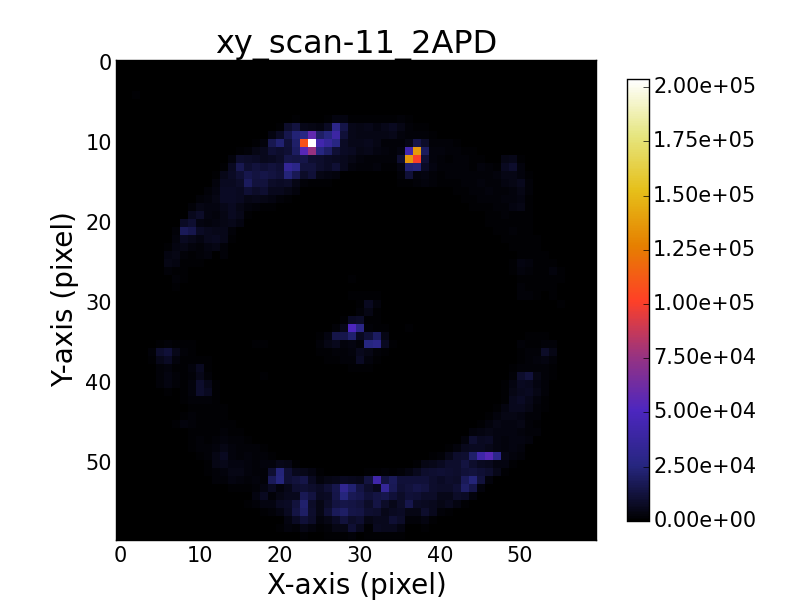
\includegraphics[trim = 0 0 0 0,  clip= true, width = \textwidth]{./pics/xy_scan-11_2APD.png}}
					\caption{}
					\label{subfig::antenna_laser_scan}
				\end{subfigure}
				\hfill
				\begin{subfigure}[t]{ 0.49\linewidth}
					\centering
					\testbox{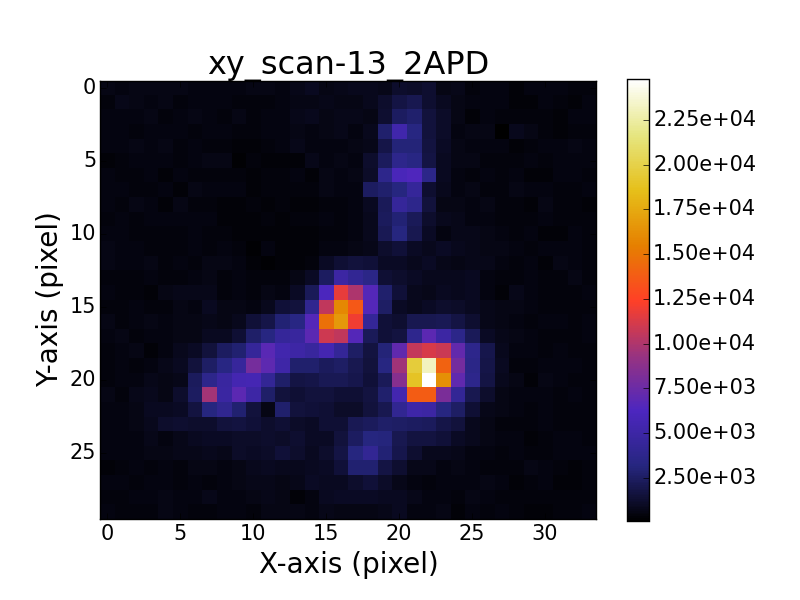
\includegraphics[trim = 0 0 0 0,  clip= true, width = \textwidth]{./pics/xy_scan-13_2APD.png}}
					\caption{
					}
					\label{subfig::antenna_bowtie_laser_scan}
				\end{subfigure}
				\caption{<caption>}
			\end{figure}

			% \begin{figure}[tp]
			% 	\centering
			% 	\testbox{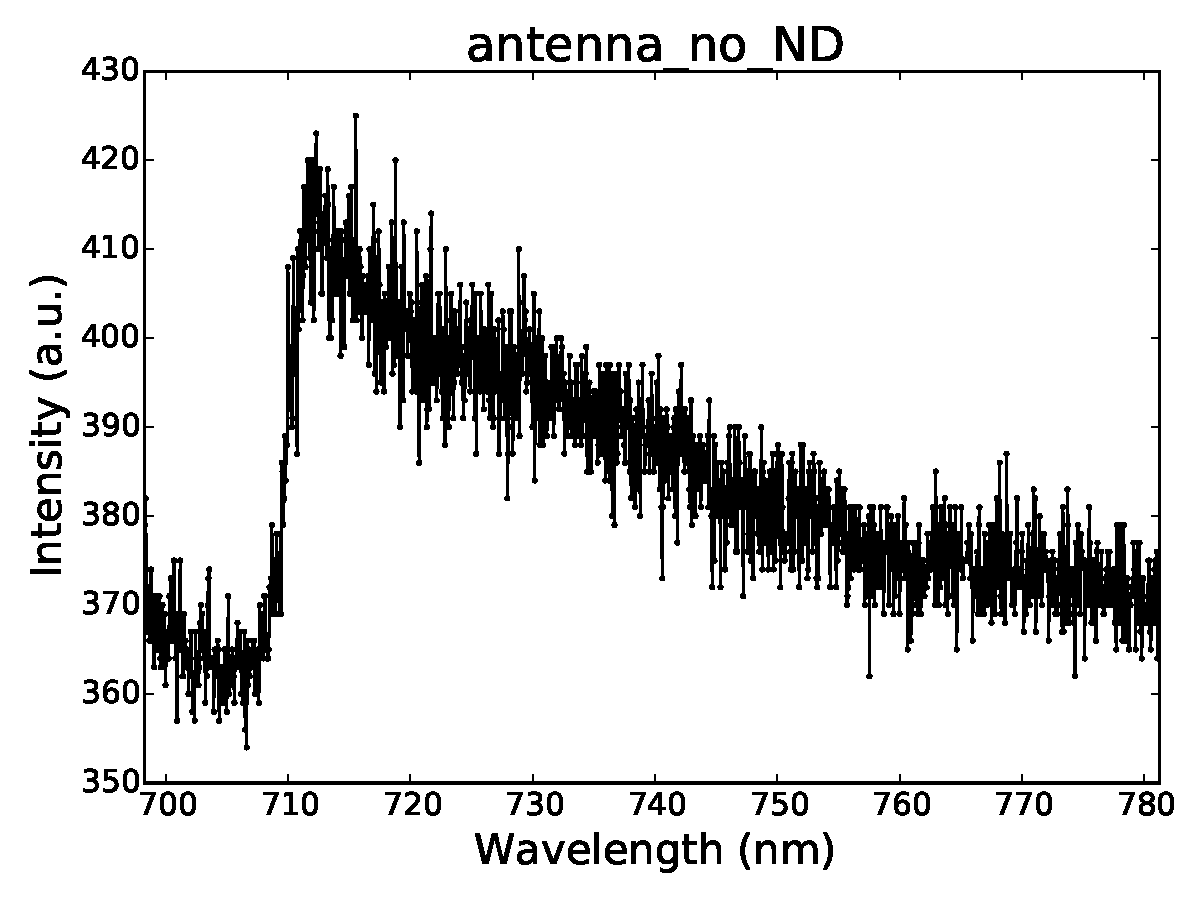
\includegraphics[trim = 0 0 0 0,  clip= true, width = 0.3\textwidth]{./pics/antenna_no_ND.pdf}}
			% 	\caption{<caption>}
			% 	\label{fig::spectrum_antenna_multiple_before}
			% \end{figure}

			\begin{figure}[tp]
				\begin{subfigure}[t]{ 0.49\linewidth}
					\centering
					\testbox{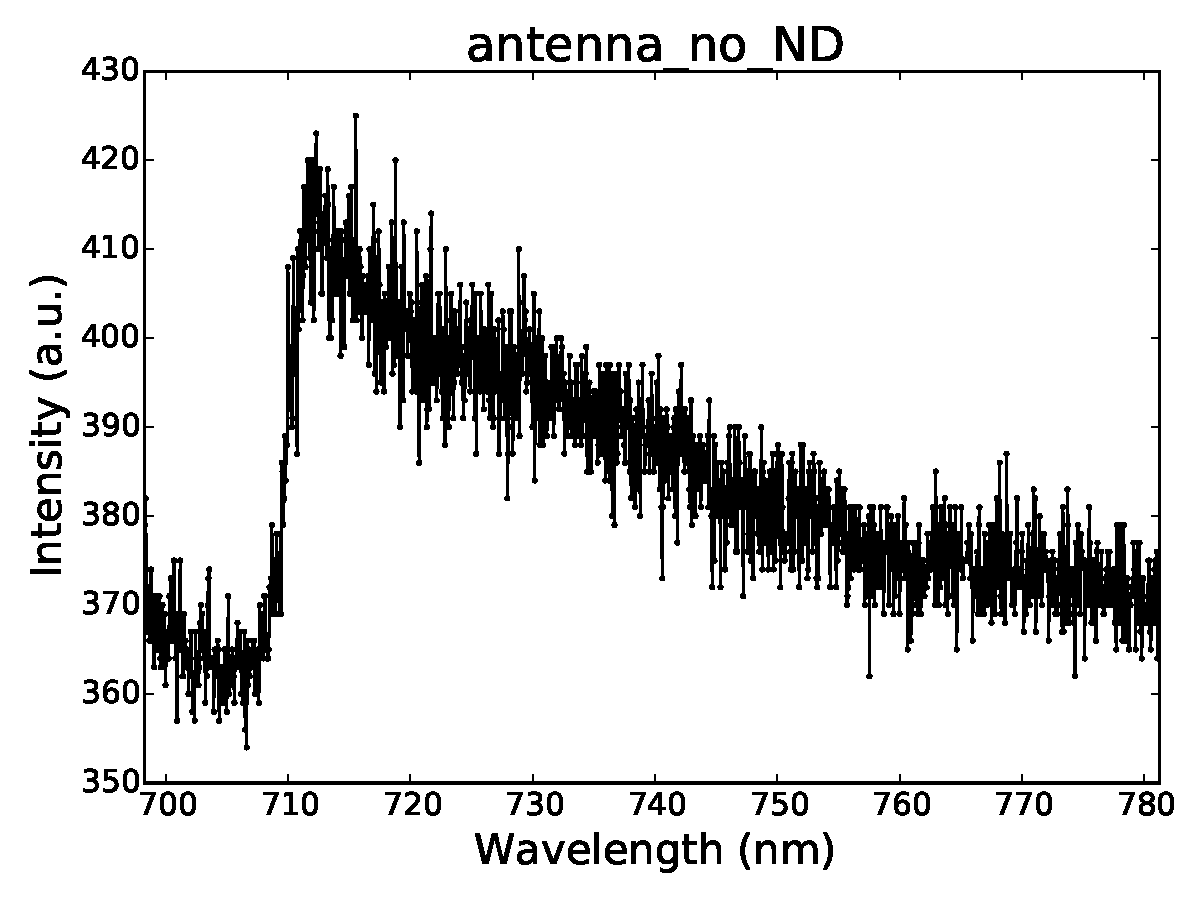
\includegraphics[trim = 0 0 0 0,  clip= true, width = \textwidth]{./pics/antenna_no_ND.pdf}}
					\caption{}
					\label{subfig::spectrum_antenna_no_nd}
				\end{subfigure}
				\hfill
				\begin{subfigure}[t]{ 0.49\linewidth}
					\centering
					\testbox{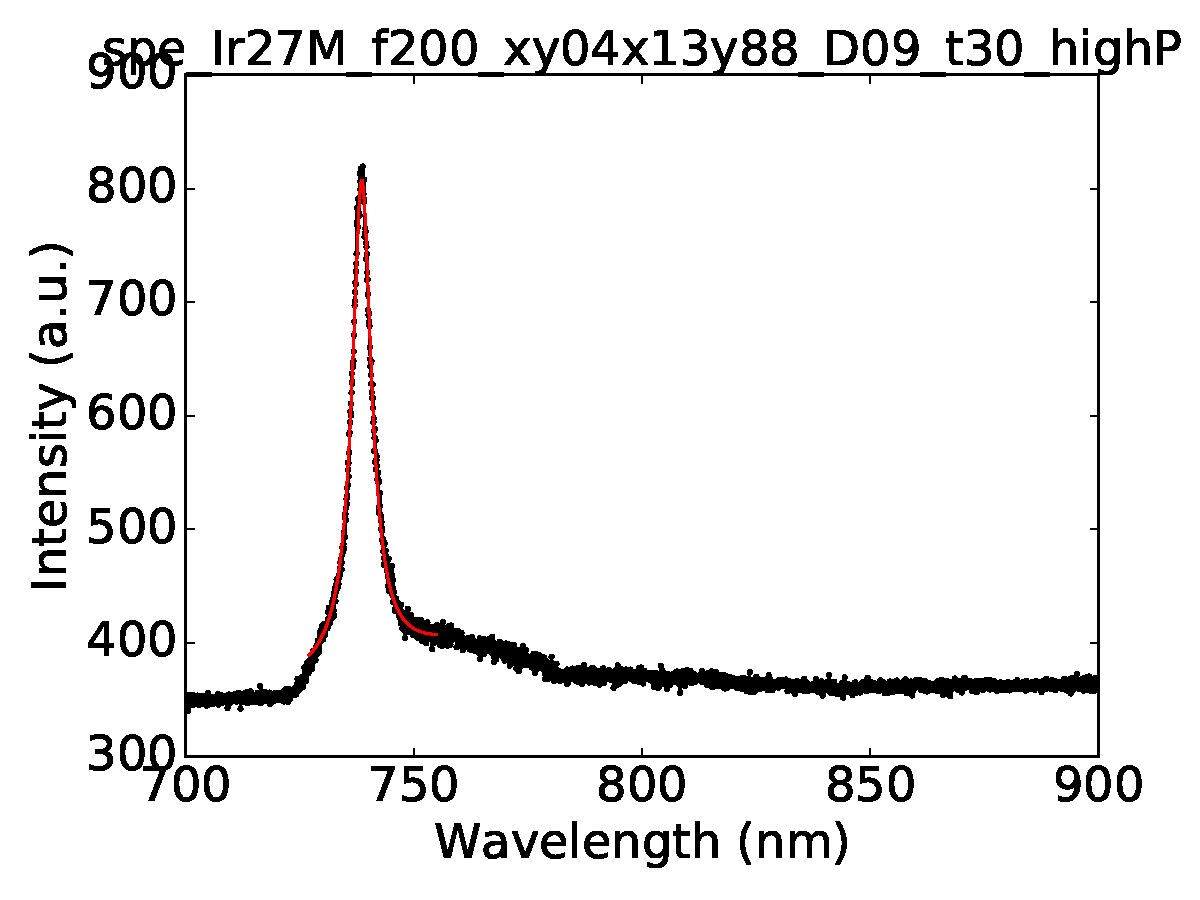
\includegraphics[trim = 0 0 0 0,  clip= true, width = \textwidth]{./pics/spe_Ir27M_f200_xy04x13y88_D09_t30_highP_fit.pdf}}
					\caption{}
					\label{subfig::spectrum_nd_multiple}
				\end{subfigure}
				\caption{<caption>}
			\end{figure}

			\begin{figure}[tp]
				\begin{subfigure}[t]{ 0.49\linewidth}
					\centering
					\testbox{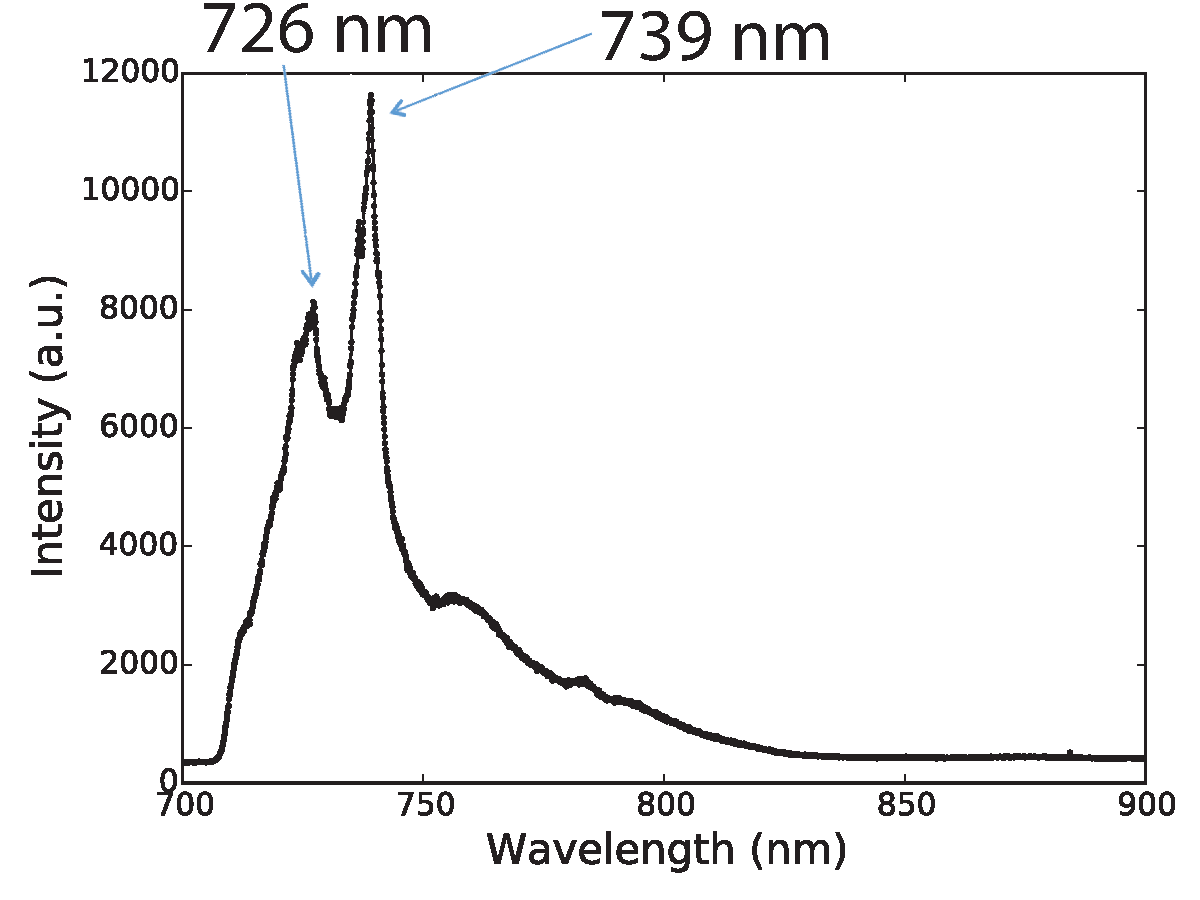
\includegraphics[trim = 0 0 0 0,  clip= true, width = \textwidth]{./pics/find_middle_with_ccd_highP_2_arrows.pdf}}
					\caption{}
					\label{subfig::spectrum_antenna_nd_multiple}
				\end{subfigure}
				\hfill
				\begin{subfigure}[t]{ 0.49\linewidth}
					\centering
					\testbox{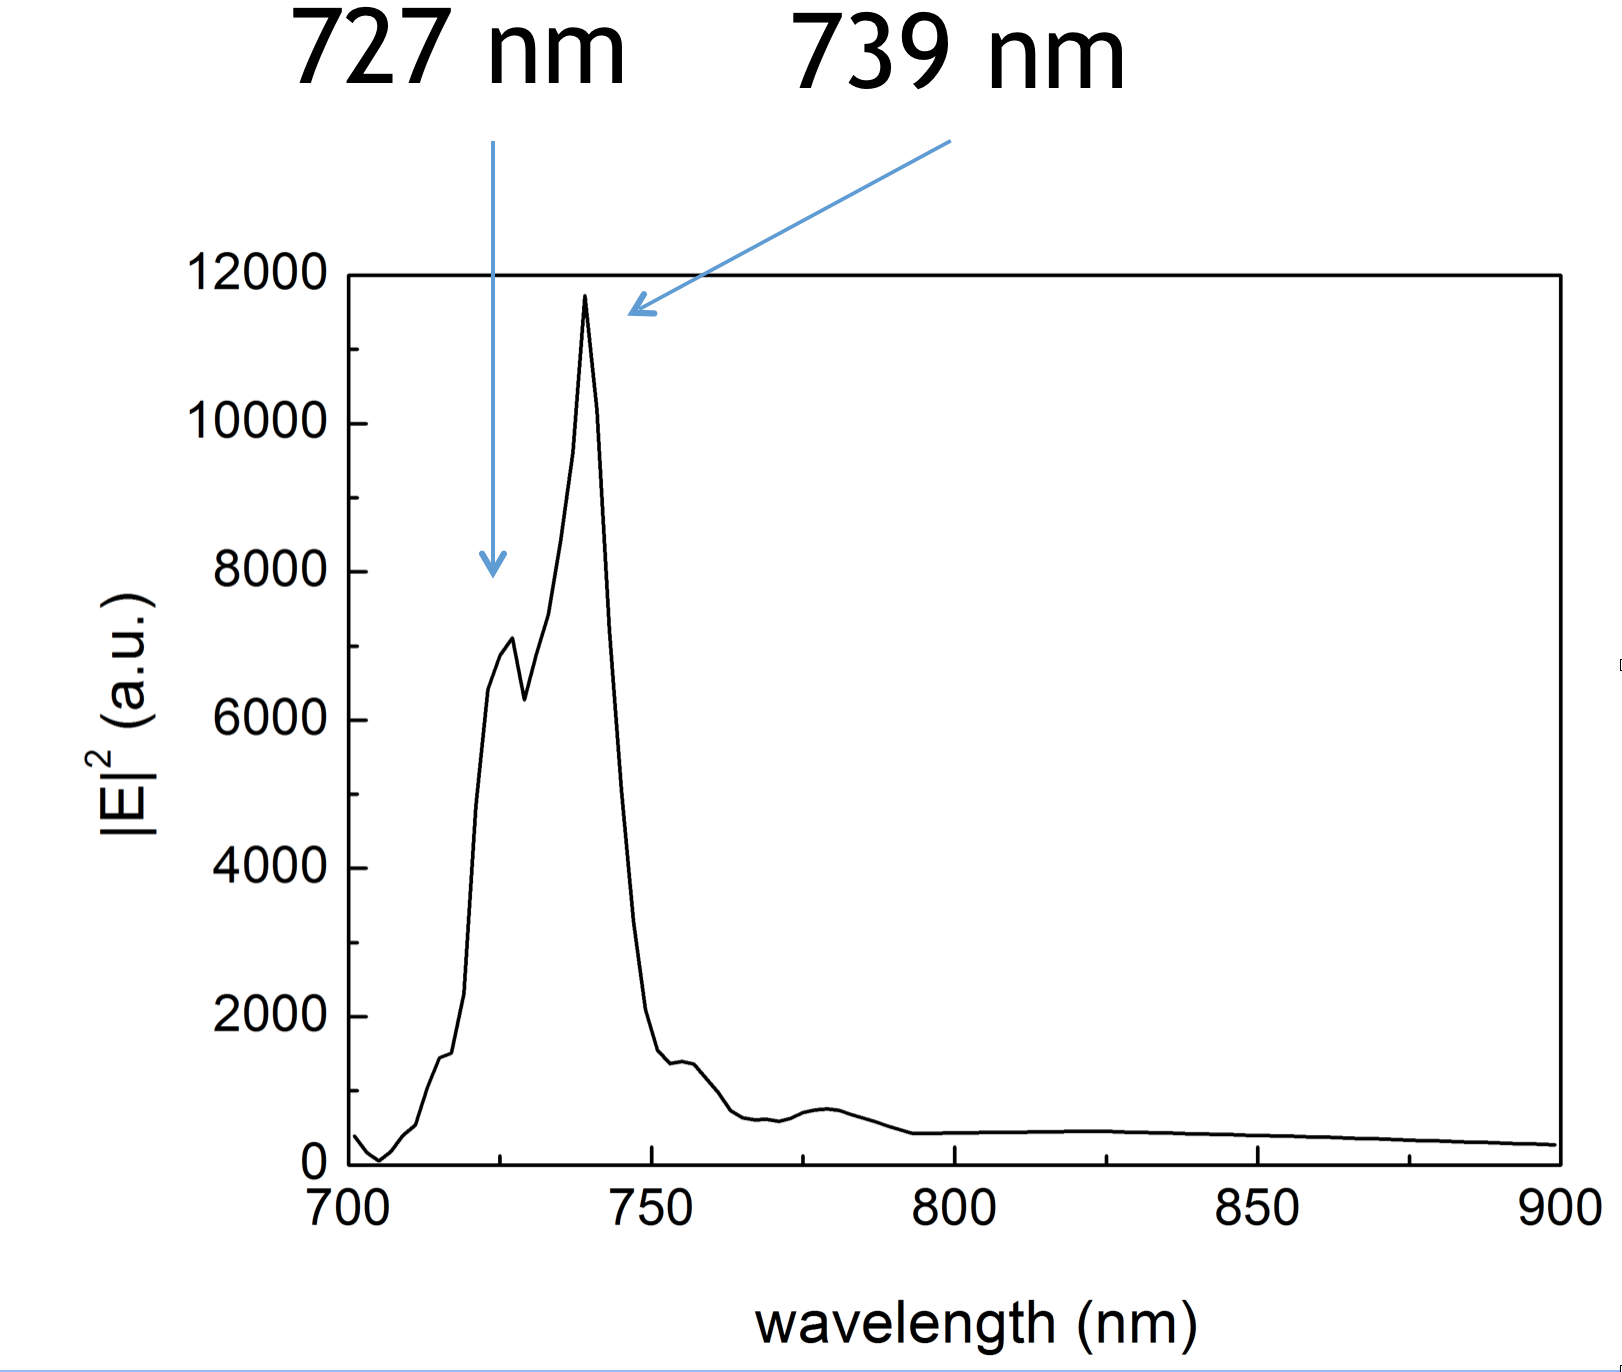
\includegraphics[trim = 0 0 0 0,  clip= true, width = \textwidth]{./pics/antenna_convolution.png}}
					\caption{}
					\label{subfig::antenna_convolution}
				\end{subfigure}
				\caption{<caption>}
			\end{figure}

		\subsubsection{\Nd With Single \siv Coupled to Antenna}

			\begin{figure}[tp]
				\begin{subfigure}[t]{ 0.49\linewidth}
					\centering
					\testbox{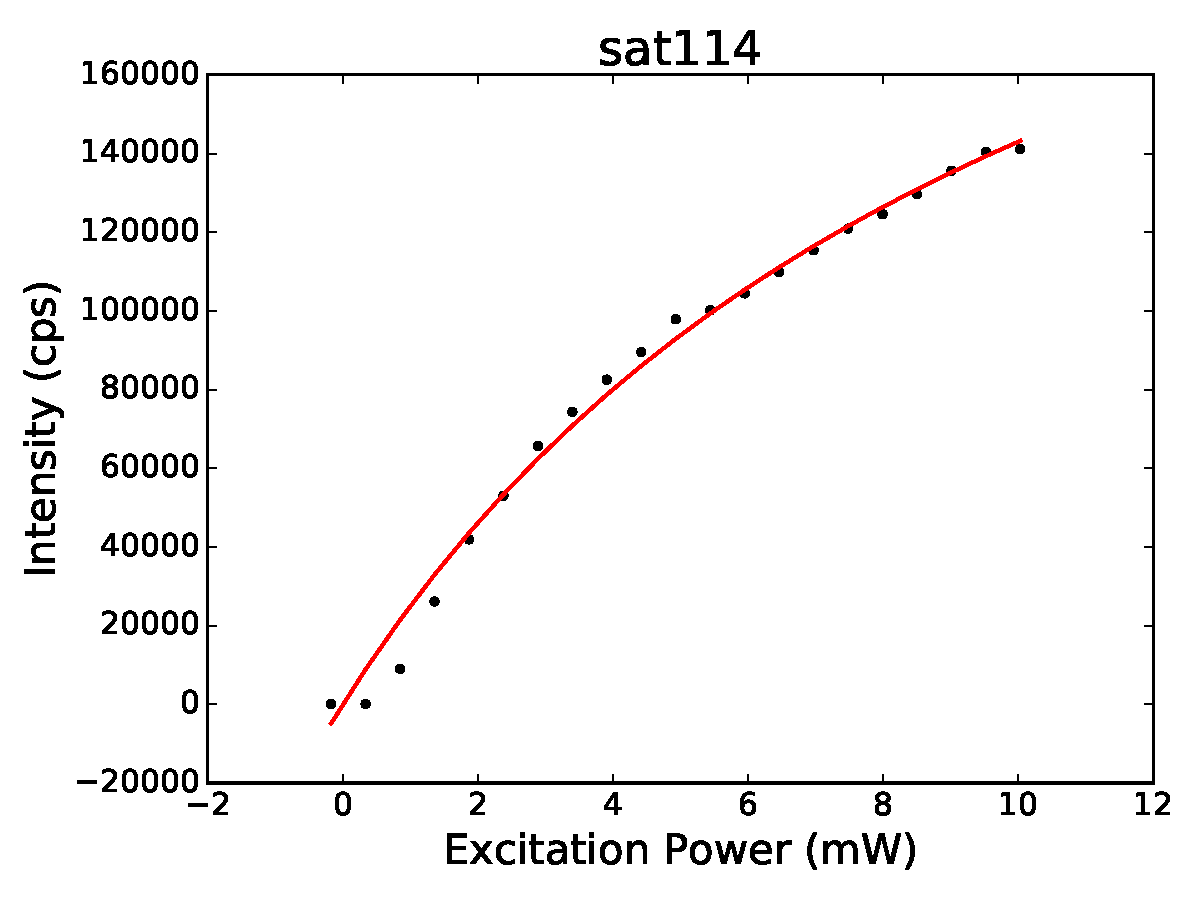
\includegraphics[trim = 0 0 0 0,  clip= true, width = \textwidth]{./pics/sat114_fit_bkg.pdf}}
					\caption{}
					\label{subfig::single_siv_sat_before_transfer_antenna}
				\end{subfigure}
				\hfill
				\begin{subfigure}[t]{ 0.49\linewidth}
					\centering
					\testbox{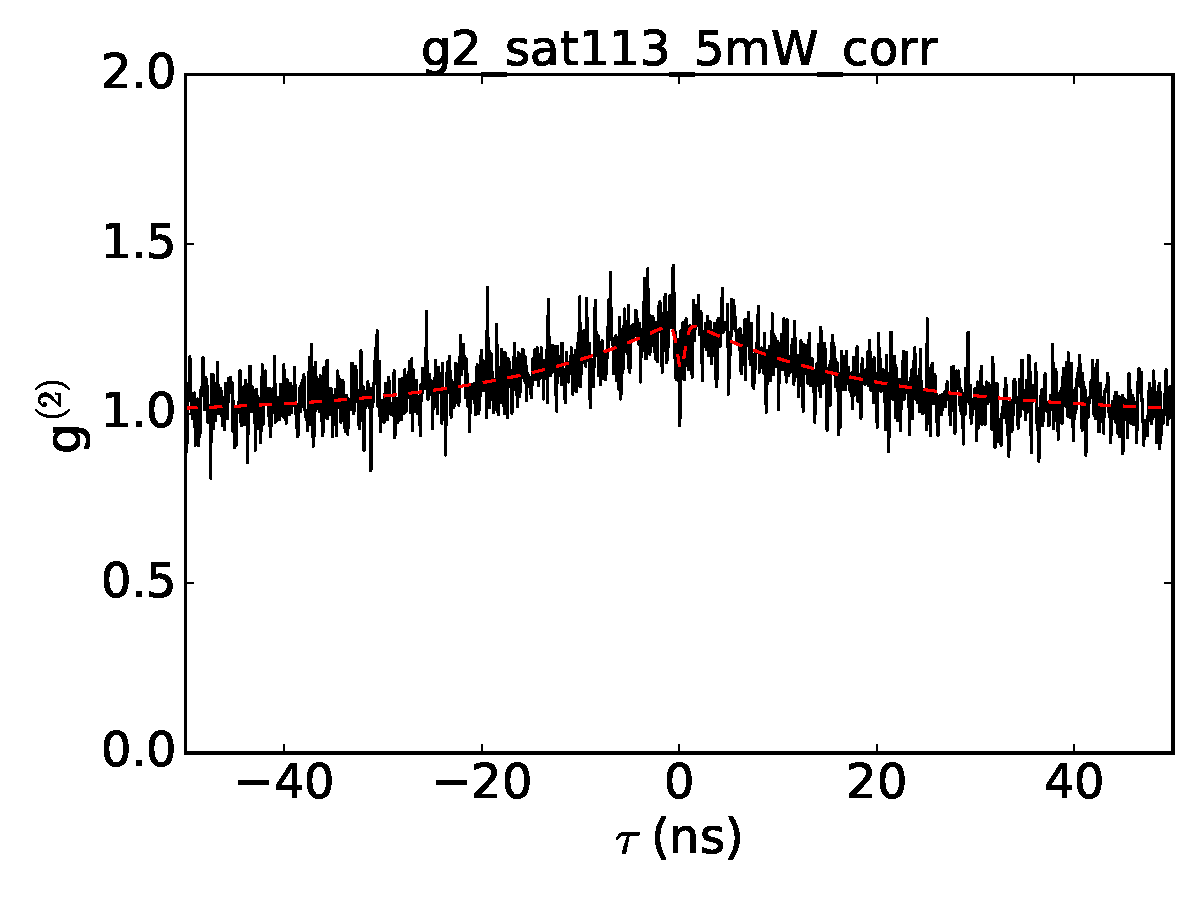
\includegraphics[trim = 0 0 0 0,  clip= true, width = \textwidth]{./pics/g2_sat113_5mW_corr_fit.pdf}}
					\caption{}
					\label{subfig::single_siv_g2_before_transfer_antenna}
				\end{subfigure}
				\caption{<caption>}
			\end{figure}

			\begin{figure}[tp]
				\begin{subfigure}[t]{ 0.49\linewidth}
					\centering
					\testbox{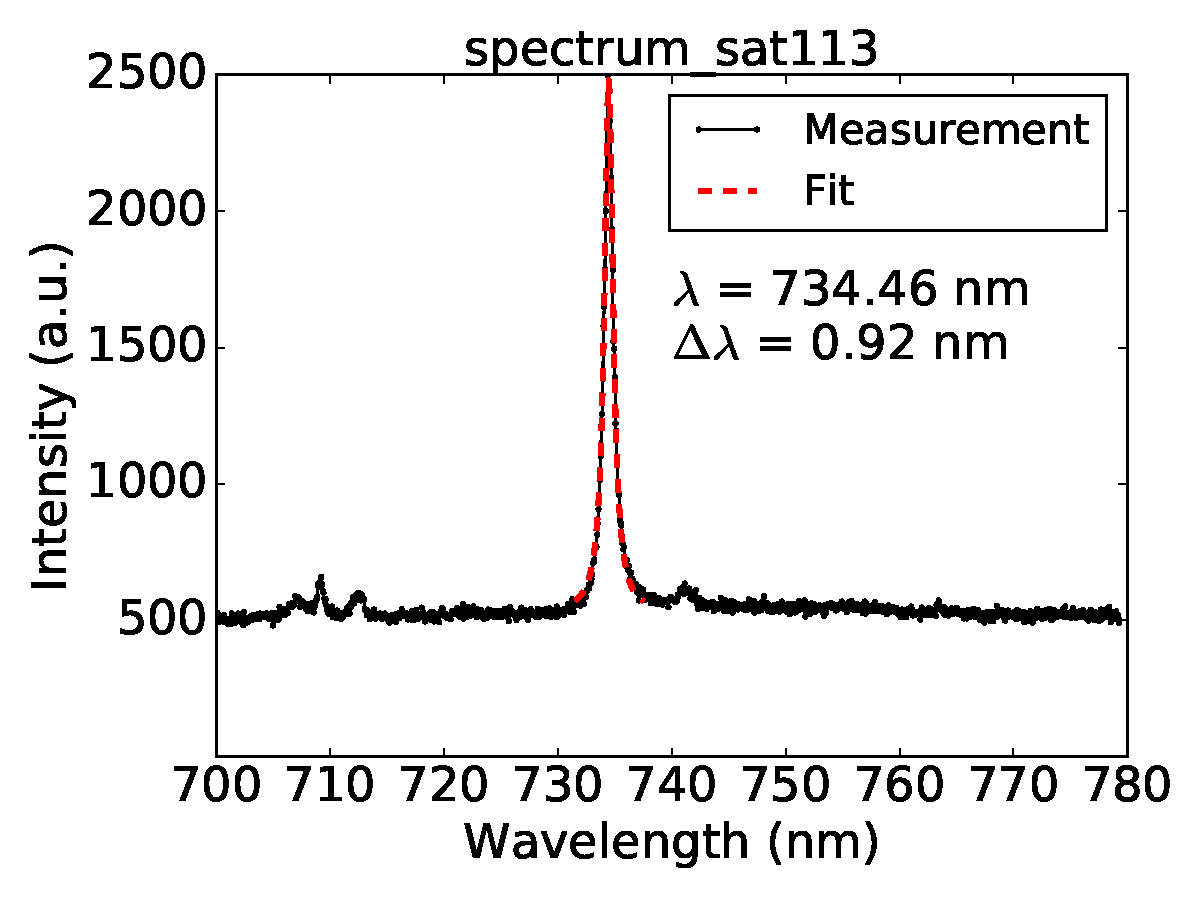
\includegraphics[trim = 0 0 0 0,  clip= true, width = \textwidth]{./pics/single_spectrum_sat113_fit.pdf}}
					\caption{}
					\label{subfig::single_siv_spec_before_transfer_antenna}
				\end{subfigure}
				\hfill
				\begin{subfigure}[t]{ 0.49\linewidth}
					\centering
					\testbox{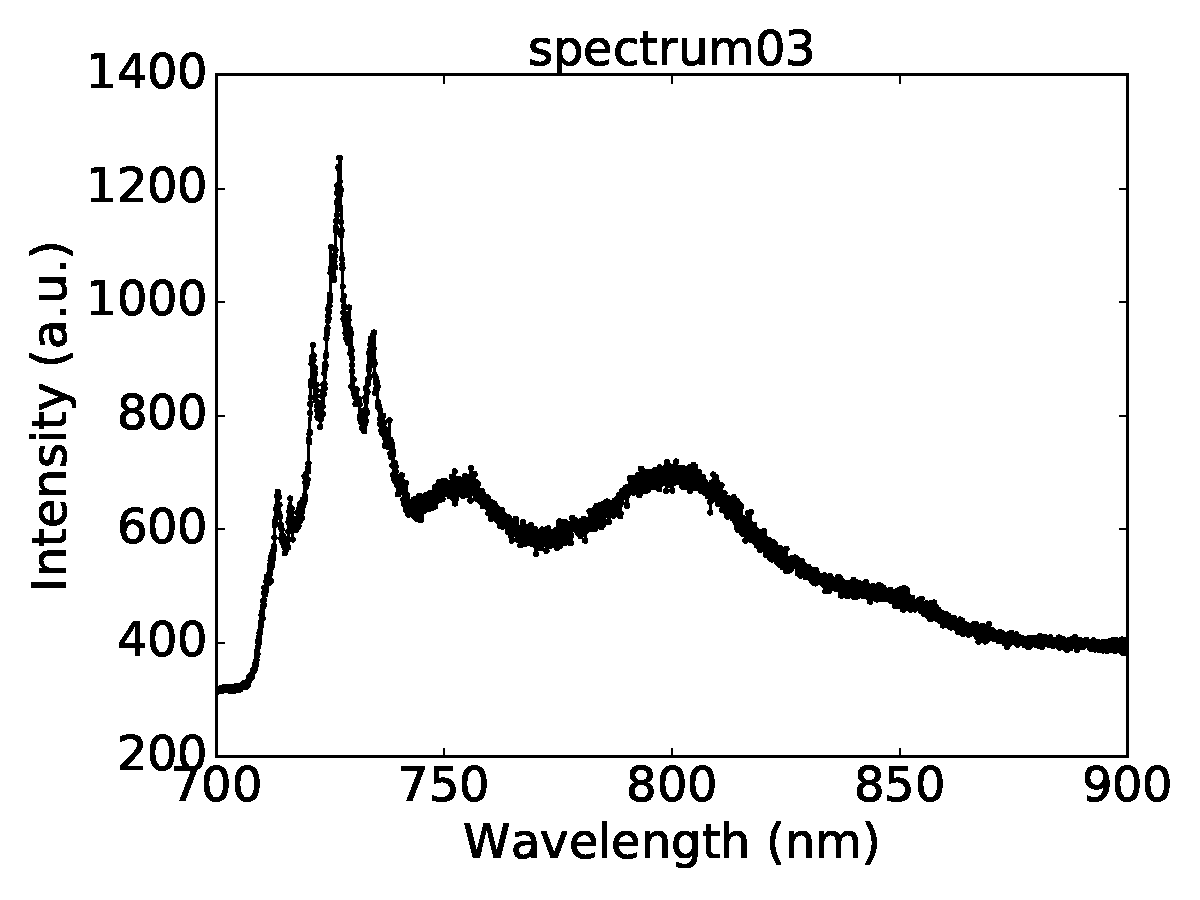
\includegraphics[trim = 0 0 0 0,  clip= true, width = \textwidth]{./pics/spectrum03.pdf}}
					\caption{}
					\label{subfig::single_siv_spec_after_transfer_antenna}
				\end{subfigure}
				\caption{<caption>}
			\end{figure}

			\begin{figure}[tp]
				\begin{subfigure}[t]{ 0.49\linewidth}
					\centering
					\testbox{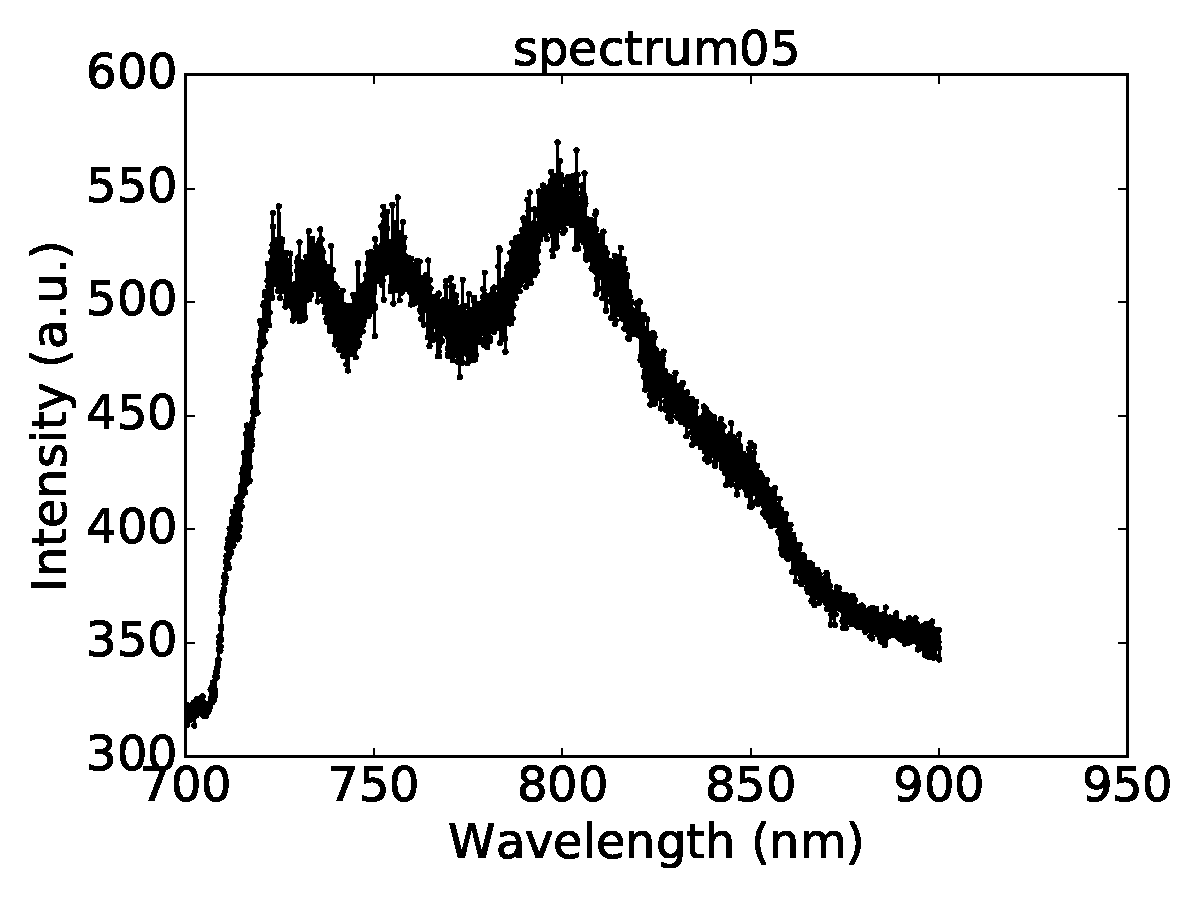
\includegraphics[trim = 0 0 0 0,  clip= true, width = \textwidth]{./pics/spectrum05.pdf}}
					\caption{}
					\label{subfig::single_siv_spec_bkg_antenna}
				\end{subfigure}
				\hfill
				\begin{subfigure}[t]{ 0.49\linewidth}
					\centering
					\testbox{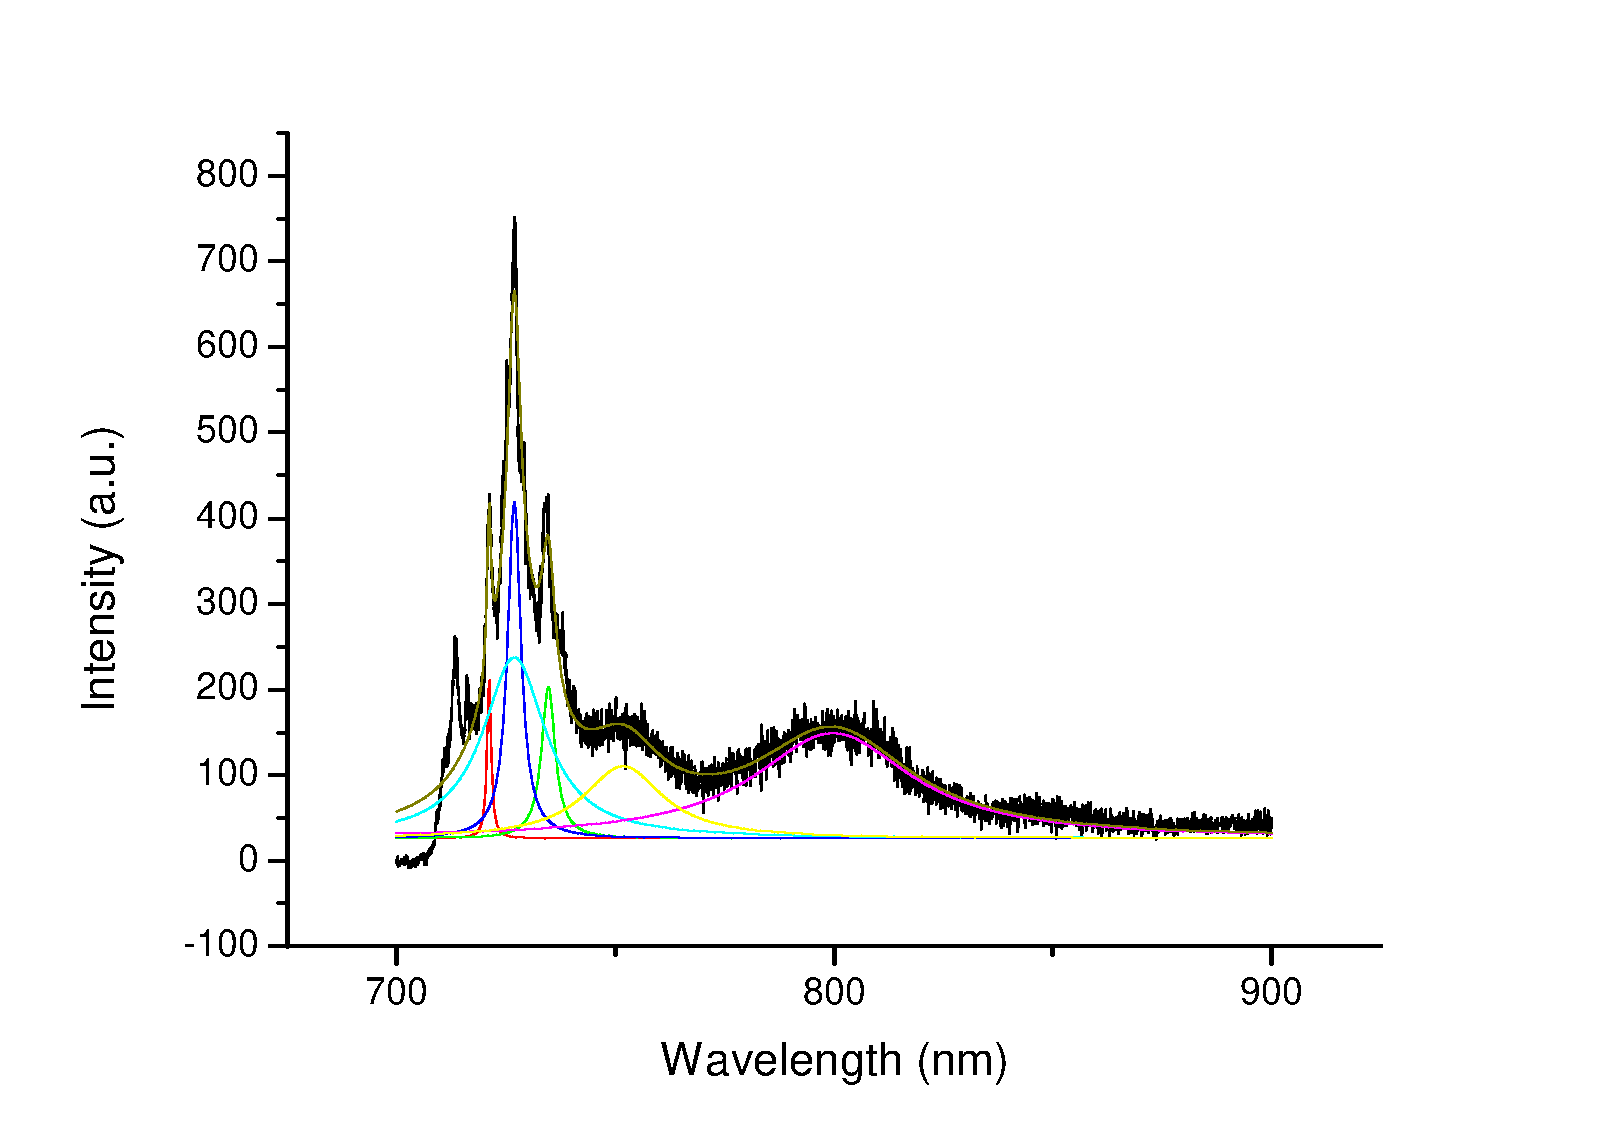
\includegraphics[trim = 0 0 0 0,  clip= true, width = \textwidth]{./pics/spectrum_sat113_fit_origin.pdf}}
					\caption{}
					\label{subfig::single_siv_spec_after_transfer_antenna_bkg_corrected}
				\end{subfigure}
				\caption{<caption>}
			\end{figure}
